% This is text associated with the open textbook "Open Electromagnetics"
% See immediately below for author, date
% <License info goes here (boilerplate, not read by project compiler)>

%ORB TITLE Fundamentals of Waves  
%ORB AUTHOR 0       # S.W. Ellingson, Virginia Tech (ellingson@vt.edu)
%ORB DATE   20180731
%ORB ABSTRACT 

\label{m0074_Fundamentals_of_Waves} % <-- Must match name of this file and module directory name.  Don't mess with this!
\index{waves!fundamentals|(}

In this section, we formally introduce the concept of a wave and explain some basic characteristics.

To begin, let us consider not electromagnetic waves, but rather sound waves.  
To be clear, sound waves 
\index{sound (waves)}
and electromagnetic waves are completely distinct phenomena. Sound waves are variations in pressure, whereas electromagnetic waves are variations in electric and magnetic fields.
However, the mathematics that govern sound waves and electromagnetic waves are very similar, so the analogy provides useful insight.
Furthermore, sound waves are intuitive for most people because they are readily observed.   
So, here we go:

Imagine standing in an open field and that it is completely quiet.
In this case, the air pressure everywhere is about 101~kPa (101,000 N/m$^2$) at sea level, % 101.325, https://en.wikipedia.org/wiki/Atmospheric_pressure
and we refer to this as the \emph{quiescent air pressure}.
Sound can be described as the \emph{differential air pressure} $p(x,y,z,t)$, which we define as the absolute air pressure at the spatial coordinates $(x,y,z)$ minus the quiescent air pressure. 
So, when there is no sound, $p(x,y,z,t)=0$.
The function $p$ as an example of a  \emph{scalar field}.\footnote{Although it's not important in this section, you can read about the concept of a ``field'' in Section~\ref{m0001_What_is_a_Field}.}
\index{field!scalar}
\index{scalar field|see {field, scalar}}

Let's also say you are standing at $x=y=z=0$ and you have brought along a friend who is standing at $x=d$; i.e., a distance $d$ from you along the $x$ axis.
Also, for simplicity, let us consider only what is happening along the $x$ axis; i.e., $p(x,t)$.

At $t=0$, you clap your hands once.
This forces the air between your hands to press outward, creating a region of increased pressure (i.e., $p>0$) that travels outward.  
As the region of increased pressure moves outward, it leaves behind a region of low pressure where $p<0$.
Air molecules immediately move toward this region of lower pressure, and so the air pressure quickly returns to the quiescent value, $p=0$.
The traveling disturbance in $p(x,t)$ is the sound of the clap.
The disturbance continues to travel outward until it reaches your friend, who then hears the clap. 

At each point in time, you can make a plot of $p(x,t)$ versus $x$ for the current value of $t$.
This is shown in Figure~\ref{m0074_fClap}.
At times $t<0$, we have simply $p(x,t)=0$.
A short time after $t=0$, the peak pressure is located at slightly to the right of $x=0$.
The pressure is not a simple impulse because interactions between air molecules constrain the pressure to be continuous over space.
So instead, we see a rounded pulse representing the rapid build-up and similarly rapid decline in air pressure.
A short time later $p(x,t)$ looks very similar, except the pulse is now further away.
%
\begin{figure}
\begin{center}
\pdftooltip{{  % note double braces
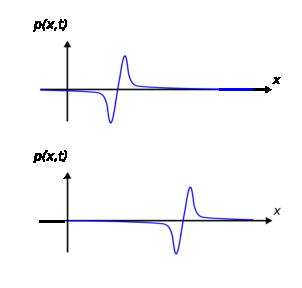
\includegraphics[width=2.5in]{modules/m0074_fClap.eps}
}}{The figure shows two x-y plots, one above the other. Differential pressure is on the y-axis and distance is on the x-axis. In each graph, the area of increased pressure is represented by one period of an approximately-sinusoidal waveform. The bottom graph shows the waveform farther away on the x-axis than the top graph.}
\end{center} 
%\vspace{2in}
% https://commons.wikimedia.org/wiki/File:M0074_fClap.svg
\centerline{\scriptsize 
\copyright~\hyperref[m0074_fClap_Credit]{Y.\ Qin} 
\href{https://creativecommons.org/licenses/by/4.0/}{CC BY 4.0} 
} 
\caption{
\label{m0074_fClap}
The differential pressure $p(x,t)$ (\emph{top}) a short time after the clap and (\emph{bottom}) a slightly longer time after the clap.
}
\end{figure}

Now: What precisely is $p(x,t)$?
% https://en.wikipedia.org/wiki/Acoustic_wave_equation
Completely skipping over the derivation, the answer is that $p(x,t)$ is the solution to the \emph{acoustic wave equation} 
\index{wave equation!acoustic}
\index{acoustic wave equation|see {wave equation, acoustic}}
(see ``Additional References'' at the end of this section):
%
\begin{equation}
\frac{\partial^2 p}{\partial x^2} - \frac{1}{c_s^2}\frac{\partial^2 p}{\partial t^2} = 0
\label{m0074_eAcousticWaveEquation}
\end{equation}
%
where $c_s$ is the speed of sound, which is about 340~m/s at sea level. % https://en.wikipedia.org/wiki/Speed_of_sound
Just to emphasize the quality of the analogy between sound waves and electromagnetic waves, know that the acoustic wave equation is mathematically identical to equations that that govern electromagnetic waves.

Although ``transient'' phenomena -- analogous to a clap -- are of interest in electromagnetics, an even more common case of interest is the wave resulting from a sinusoidally-varying source.  We can demonstrate this kind of wave in the context of sound as well.
Here we go: 

In the previous scenario, you pick up a trumpet and blow a perfect A note.
The A note is 440~Hz, meaning that the air pressure emerging from your trumpet is varying sinusoidally at a frequency of 440~Hz.
Let's say you can continue to blow this note long enough for the entire field to be filled with the sound of your trumpet.
Now what does the pressure-versus-distance curve look like?
Two simple observations will settle that question:
%
\begin{itemize}
\item $p(x,t)$ at any \emph{constant position} $x$ is a sinusoid as a function of $x$.  
This is because the acoustic wave equation is linear and time invariant, so a sinusoidal excitation (i.e., your trumpet) results in a sinusoidal response at the same frequency (i.e., the sound heard by your friend).
\item $p(x,t)$ at any \emph{constant time} $t$ is also a sinusoid as a function of $x$.
This is because the sound is propagating away from the trumpet and toward your friend, and anyone in between will also hear the A note, but with a phase shift determined by the difference in distances.
\end{itemize}
%
This is enough information to know that the solution must have the form:
%
\begin{equation}
p(x,t) = A_m \cos\left( \omega t - \beta x + \psi \right)
\label{m0074_eGenericWave}
\end{equation} 
%
where $\omega = 2\pi f$, $f=440$~Hz, and $A_m$, $\beta$, and $\psi$ remain to be determined.

You can readily verify that Equation~\ref{m0074_eGenericWave} satisfies the acoustic wave equation when
%
\begin{equation}
\beta = \frac{\omega}{c_s}
\end{equation}
%
In this problem, we find $\beta\cong 8.13$~rad/m. 
This means that at any given time, the difference in phase measured between any two points separated by a distance of 1~m is 8.13~rad.
The parameter $\beta$ goes by at least three names: \emph{phase propagation constant}, 
\index{propagation constant!phase}
\emph{wavenumber}, 
and \emph{spatial frequency}.
\index{spatial frequency}
The term ``spatial frequency'' is particularly apt, since $\beta$ plays precisely the same role for distance ($x$) as $\omega$ plays for time ($t$) -- This is apparent from Equation~\ref{m0074_eGenericWave}.
However, ``wavenumber'' is probably the more commonly-used term.

%ORB HIGHLIGHT
\begin{mdframed}[backgroundcolor=yellow!20,nobreak=true] 
The wavenumber 
\index{wavenumber}
$\beta$ (rad/m) is the rate at which the phase of a sinusoidal wave progresses with distance.   
\end{mdframed}

Note that $A_m$ and $\psi$ are not determined by the wave equation, but instead are properties of the source.
Specifically, $A_m$ is determined by how hard we blow, and $\psi$ is determined by the time at which we began to blow and the location of the trumpet.
For simplicity, let us assume that we begin to blow at time $t\ll 0$; i.e., in the distant past so that the sound pressure field has achieved steady state by $t=0$.
Also, let us set $\psi=0$ and set $A_m=1$ in whatever units we choose to express $p(x,t)$.
We then have:
%
\begin{equation}
p(x,t) = \cos\left( \omega t - \beta x \right)
\label{m0074_eSimpleWave}
\end{equation} 
%
Now we have everything we need to make plots of $p(x)$ at various times.

Figure~\ref{m0074_fTrumpet}(a) shows $p(x,t=0)$.
As expected, $p(x,t=0)$ is periodic in $x$.  
The associated period is referred to as the \emph{wavelength} $\lambda$.
Since $\lambda$ is the distance required for the phase of the wave to increase by $2\pi$~rad, and because phase is increasing at a rate of $\beta$ rad/m, we find:
%
\begin{equation}
\lambda = \frac{2\pi}{\beta}
\end{equation}
%
In the present example, we find $\lambda\cong 77.3$~cm.
%
\begin{figure}
\begin{center}
\pdftooltip{{  % note double braces
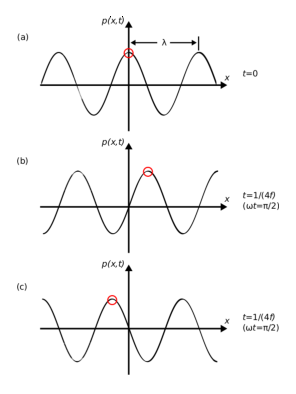
\includegraphics[width=2.9in]{modules/m0074_fTrumpet.eps}
}}{The figure shows three graphs: (a) is above (b) which is above (c). The three graphs have sinusoidal waves of identical wavelengths and amplitudes. In (a), a red circle pinpoints the peak of the wave which coincides with the y-intercept. In (b), this same peak is a quarter wavelength to the right of the y-axis. In (c), it is a quarter wavelength to the left of the y-axis.}
\end{center} 
%\vspace{2in}
% https://commons.wikimedia.org/wiki/File:M0074_fTrumpet.svg
\centerline{\scriptsize 
\copyright~\hyperref[m0074_fTrumpet_Credit]{Y.\ Qin} 
\href{https://creativecommons.org/licenses/by/4.0/}{CC BY 4.0} 
} 
\caption{
\label{m0074_fTrumpet}
The differential pressure $p(x,t)$ for 
(a) $t=0$,
(b) $t=1/4f$ for ``$-\beta x$,'' as indicated in Equation~\ref{m0074_eSimpleWave} (wave traveling to right); and
(c) $t=1/4f$ for ``$+\beta x$'' (wave traveling to left).
}
\end{figure}

%ORB HIGHLIGHT
\begin{mdframed}[backgroundcolor=yellow!20,nobreak=true]
Wavelength 
\index{wavelength}
$\lambda=2\pi/\beta$ is the distance required for the phase of a sinusoidal wave to increase by one complete cycle (i.e., $2\pi$ rad) at any given time. 
\end{mdframed}

Now let us consider the situation at $t=+1/4f$, which is $t=568~\mu$s and $\omega t=\pi/2$.
We see in Figure~\ref{m0074_fTrumpet}(b) that the waveform has shifted a distance $\lambda/4$ to the right.
It is in this sense that we say the wave is propagating in the $+x$ direction.
Furthermore, we can now compute a \emph{phase velocity} $v_p$: 
We see that a point of constant phase has shifted a distance $\lambda/4$ in time $1/4f$, so   
%
\begin{equation}
v_p = \lambda f 
\end{equation}
%
In the present example, we find $v_p\cong 340$~m/s; i.e., we have found that the phase velocity is equal to the speed of sound $c_s$.  
It is in this sense that we say that the phase velocity is the speed at which the wave propagates.\footnote{It is worth noting here is that ``velocity'' is technically a vector; i.e., speed in a given direction. Nevertheless, this quantity is actually just a speed, and this particular abuse of terminology is generally accepted.}

%ORB HIGHLIGHT
\begin{mdframed}[backgroundcolor=yellow!20,nobreak=true]
Phase velocity 
\index{phase velocity}
$v_p=\lambda f$ is the speed at which a point of constant phase in a sinusoidal waveform travels.  
\end{mdframed}

Recall that in Equation~\ref{m0074_eGenericWave} we declared that $\beta x$ is subtracted from the argument of the sinusoidal function.  
To understand why, let's change the sign of $\beta x$ and see if it still satisfies the wave equation -- one finds that it does.
Next, we repeat the previous experiment and see what happens.
The result is shown in Figure~\ref{m0074_fTrumpet}(c).
Note that points of constant phase have traveled an equal distance, but now in the $-x$ direction.  
In other words, this alternative choice of sign for $\beta x$ within the argument of the cosine function represents a wave that is propagating in the opposite direction.  
This leads us to the following realization:

%ORB HIGHLIGHT
\begin{mdframed}[backgroundcolor=yellow!20,nobreak=true]
If the phase of the wave is decreasing with $\beta x$, then the wave is propagating in the $+x$ direction.
If the phase of the wave is increasing with $\beta x$, then the wave is propagating in the $-x$ direction.
\end{mdframed}

Since the prospect of sound traveling toward the trumpet is clearly nonsense in the present situation, we may neglect the latter possibility.
However, what happens if there is a wall located in the distance, behind your friend?
Then, we expect an echo from the wall, which would be a second wave propagating in the reverse direction and for which the argument of the cosine function would contain the term ``$+\beta x$.''

Finally, let us return to electromagnetics.  
Electromagnetic waves satisfy precisely the same wave equation (i.e., Equation~\ref{m0074_eAcousticWaveEquation}) as do sound waves, except that the phase velocity is much greater.
Interestingly, though, the frequencies of electromagnetic waves are also much greater than those of sound waves, so we can end up with wavelengths having similar orders of magnitude.
In particular, an electromagnetic wave with $\lambda=77.3$~cm (the wavelength of the ``A'' note in the preceding example) lies in the radio portion of the electromagnetic spectrum.

An important difference between sound and electromagnetic waves is that electromagnetic waves are vectors; that is, they have \emph{direction} as well as magnitude.
Furthermore, we often need to consider multiple electromagnetic vector waves (in particular, both the \emph{electric field} and the \emph{magnetic field}) in order to completely understand the situation.
Nevertheless the concepts of wavenumber, wavelength, phase velocity, and direction of propagation apply in precisely the same manner to electromagnetic waves as they do to sound waves.  

{\bf Additional Reading:}
\begin{itemize}
\item ``\href{https://en.wikipedia.org/wiki/Wave_equation}{Wave Equation}'' on Wikipedia.
\item ``\href{https://en.wikipedia.org/wiki/Acoustic_wave_equation}{Acoustic Wave Equation}'' on Wikipedia.
\end{itemize}

\index{waves!fundamentals|)}












